% Reset frame number to 1
\setcounter{framenumber}{0}

% Section title slide
\begin{frame}
\frametitle{Performance Measures}
\begin{center}
\Large \textbf{Performance Measures}
\end{center}
\end{frame}

\section{Performance Measures for Classification and Regression Models}

\begin{frame}{Motivation}
  \begin{itemize}
    \item Model quality is multi-dimensional: correctness, calibration, and cost.
    \item Classification and regression differ in targets, errors, and decision rules.
    \item Data imbalance, noise, and application risk change what ``good'' means.
  \end{itemize}
\end{frame}

\begin{frame}{Problem Setup and Notation}
  \begin{itemize}
    \item Dataset: $\{(x^{(i)}, y^{(i)})\}_{i=1}^m$, predictions $\hat{y}^{(i)}$.
    \item Classification: $y^{(i)} \in \{0,1\}$ or $\{1,\dots,K\}$.
    \item Regression: $y^{(i)} \in \R$, residual $r^{(i)} = y^{(i)} - \hat{y}^{(i)}$.
    \item Outputs: deterministic labels or probabilistic scores $\hat{p}(y=1\mid x)$.
  \end{itemize}
\end{frame}

\section{Classification Performance Measures}

\begin{frame}{Confusion Matrix (Binary)}
  \begin{table}
    \centering
    \begin{tabular}{lcc}
      \toprule
      & Predicted $1$ & Predicted $0$ \\
      \midrule
      Actual $1$ & TP & FN \\
      Actual $0$ & FP & TN \\
      \bottomrule
    \end{tabular}
  \end{table}
  \vspace{0.3em}
  \begin{itemize}
    \item Defines error types and supports derived metrics.
  \end{itemize}
\end{frame}

\begin{frame}{Accuracy and Error Rate}
  \[
    \text{Accuracy} = \frac{TP + TN}{TP + FP + TN + FN}, \quad
    \text{Error} = 1 - \text{Accuracy}
  \]
  \begin{itemize}
    \item Simple and intuitive for balanced classes.
    \item Fails under class imbalance (dominant class inflates accuracy).
  \end{itemize}
\end{frame}

\begin{frame}{Precision and Recall}
  \[
    \text{Precision} = \frac{TP}{TP + FP}, \quad
    \text{Recall} = \frac{TP}{TP + FN}
  \]
  \begin{itemize}
    \item Precision: how reliable are positive predictions?
    \item Recall (TPR): how many positives are recovered?
    \item Use cases: medical screening (high recall), fraud alerts (high precision).
  \end{itemize}
\end{frame}

\begin{frame}{F1 Score}
  \[
    F_1 = \frac{2\,\text{Precision}\cdot\text{Recall}}{\text{Precision}+\text{Recall}}
  \]
  \begin{itemize}
    \item Harmonic mean penalizes extreme imbalance between precision and recall.
    \item Preferred when classes are imbalanced and both errors matter.
  \end{itemize}
\end{frame}

\begin{frame}{ROC Curve and AUC}
  \begin{itemize}
    \item TPR $= \frac{TP}{TP+FN}$, FPR $= \frac{FP}{FP+TN}$.
    \item Sweep decision threshold to trace ROC curve.
    \item Area under the ROC curve (AUC) summarizes ranking quality; $0.5$ is random.
     \[
      \text{AUC} = \int_0^1 \text{TPR}(\text{FPR}) \, d(\text{FPR})
    \]
  \end{itemize}
  \vspace{-0.2em}
  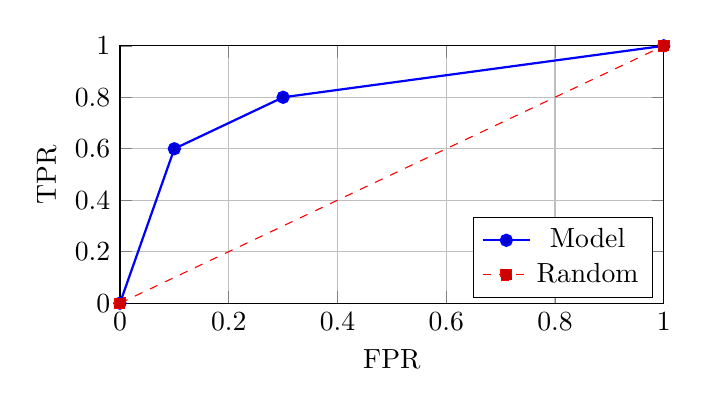
\begin{tikzpicture}
    \begin{axis}[
      width=0.7\textwidth,
      height=0.4\textwidth,
      xlabel=FPR,
      ylabel=TPR,
      xmin=0,xmax=1,ymin=0,ymax=1,
      grid=both,
      legend style={at={(0.98,0.02)},anchor=south east}
    ]
      \addplot+[thick] coordinates {(0,0) (0.1,0.6) (0.3,0.8) (1,1)};
      \addlegendentry{Model}
      \addplot+[dashed] coordinates {(0,0) (1,1)};
      \addlegendentry{Random}
    \end{axis}
  \end{tikzpicture}
\end{frame}

\begin{frame}{When ROC Can Mislead}
  \begin{itemize}
    \item With severe imbalance, FPR can appear small even with many false positives.
    \item ROC emphasizes ranking quality, not precision of positive predictions.
  \end{itemize}
\end{frame}

\begin{frame}{Precision--Recall Curve}
  \begin{itemize}
    \item Plot precision vs recall as threshold varies.
    \item More informative than ROC for rare positive class.
  \end{itemize}
  \vspace{-0.2em}
  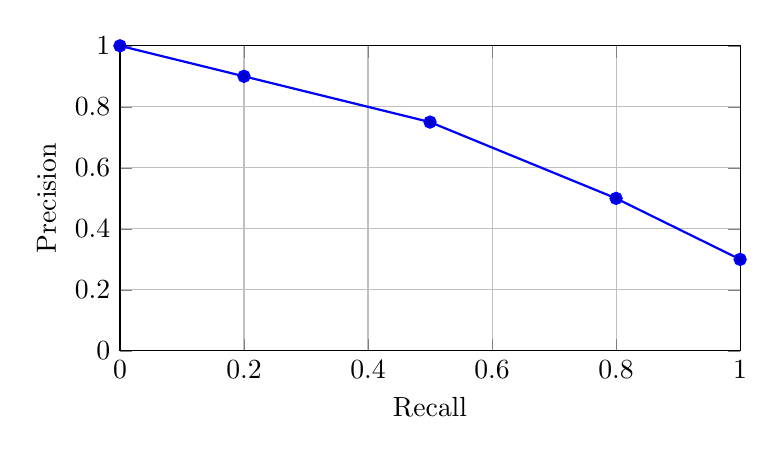
\begin{tikzpicture}
    \begin{axis}[
      width=0.78\textwidth,
      height=0.45\textwidth,
      xlabel=Recall,
      ylabel=Precision,
      xmin=0,xmax=1,ymin=0,ymax=1,
      grid=both
    ]
      \addplot+[thick] coordinates {(0.0,1.0) (0.2,0.9) (0.5,0.75) (0.8,0.5) (1.0,0.3)};
    \end{axis}
  \end{tikzpicture}
\end{frame}

\begin{frame}{Average Precision (AP)}
  \begin{itemize}
    \item AP summarizes the precision--recall curve as an area-under-curve.
    \item Common in object detection: average precision across recall levels.
    \item Interpolated form:
  \end{itemize}
  \[
    \text{AP} = \int_0^1 p_{\text{interp}}(r)\,dr, \quad
    p_{\text{interp}}(r) = \max_{\tilde{r}\ge r} p(\tilde{r})
  \]
\end{frame}

\begin{frame}{Threshold Selection}
  \begin{itemize}
    \item Decision threshold converts scores to labels; changes precision/recall.
    \item Match costs by minimizing expected error cost on validation data:
    \[
      \mathbb{E}[\text{cost}] = C_{FP}\cdot \text{FPR}\cdot (1-\pi)
      + C_{FN}\cdot \text{FNR}\cdot \pi,
    \]
    where $\pi = P(y=1)$ is the positive class rate.
    \item Use validation data and ROC/PR curves to choose an operating point.
    \item Calibrate scores (e.g., Platt scaling) before thresholding if needed.
    \item Revisit thresholds when class prevalence or costs shift over time.
  \end{itemize}
\end{frame}

\section{Regression Performance Measures}

\begin{frame}{Regression Setup}
  \begin{itemize}
    \item Targets are continuous: $y^{(i)} \in \R$.
    \item Residuals: $r^{(i)} = y^{(i)} - \hat{y}^{(i)}$.
    \item Metrics summarize magnitude and structure of residuals.
  \end{itemize}
\end{frame}

\begin{frame}{Mean Squared Error (MSE)}
  \[
    \text{MSE} = \frac{1}{m}\sum_{i=1}^m \left(y^{(i)} - \hat{y}^{(i)}\right)^2
  \]
  \begin{itemize}
    \item Penalizes large errors heavily (outlier sensitive).
    \item Natural under Gaussian noise assumption.
  \end{itemize}
\end{frame}

\begin{frame}{Root Mean Squared Error (RMSE)}
  \[
    \text{RMSE} = \sqrt{\text{MSE}}
  \]
  \begin{itemize}
    \item Same units as target variable.
    \item Easier to interpret than MSE, still outlier sensitive.
  \end{itemize}
\end{frame}

\begin{frame}{Mean Absolute Error (MAE)}
  \[
    \text{MAE} = \frac{1}{m}\sum_{i=1}^m \left|y^{(i)} - \hat{y}^{(i)}\right|
  \]
  \begin{itemize}
    \item More robust to outliers than MSE/RMSE.
    \item Linear penalty treats all deviations uniformly.
  \end{itemize}
\end{frame}

\begin{frame}{Coefficient of Determination ($R^2$)}
  \[
    R^2 = 1 - \frac{\sum_{i}(y^{(i)}-\hat{y}^{(i)})^2}{\sum_{i}(y^{(i)}-\bar{y})^2}
  \]
  \begin{itemize}
    \item Fraction of variance explained by the model.
    \item Can be negative on new data; sensitive to data range.
  \end{itemize}
\end{frame}

\begin{frame}{Visual Diagnostics}
  \begin{columns}
    \column{0.5\textwidth}
    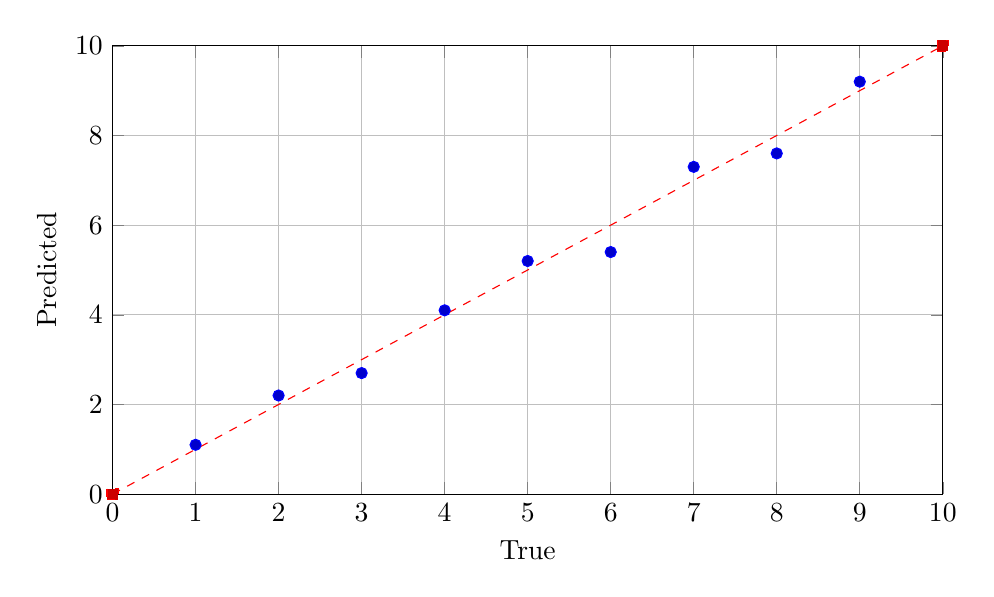
\begin{tikzpicture}
      \begin{axis}[
        width=\textwidth,
        height=0.6\textwidth,
        xlabel=True,
        ylabel=Predicted,
        xmin=0,xmax=10,ymin=0,ymax=10,
        grid=both
      ]
        \addplot+[only marks] coordinates {(1,1.1) (2,2.2) (3,2.7) (4,4.1) (5,5.2) (6,5.4) (7,7.3) (8,7.6) (9,9.2)};
        \addplot+[dashed] coordinates {(0,0) (10,10)};
      \end{axis}
    \end{tikzpicture}
    \column{0.5\textwidth}
    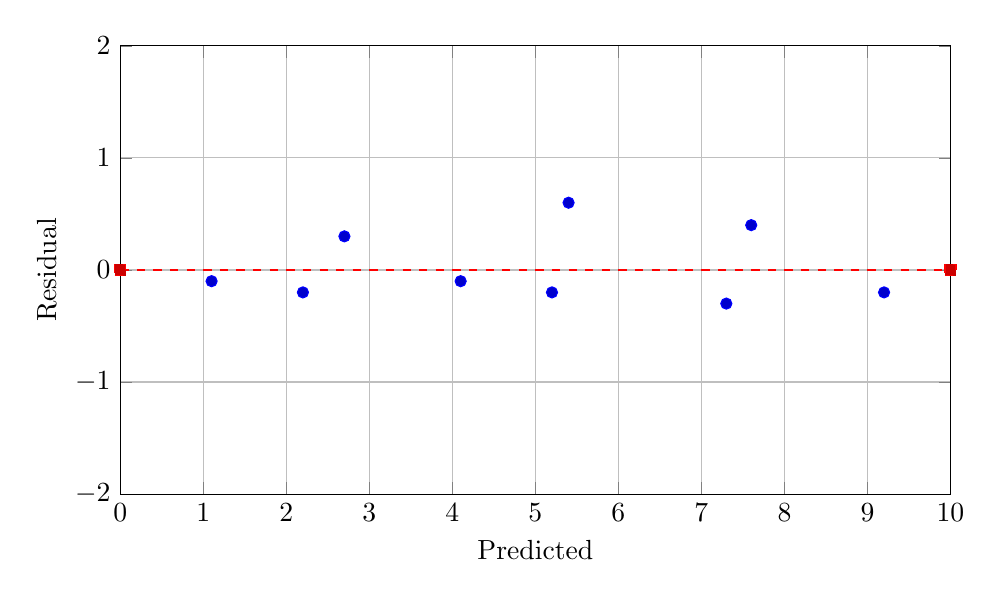
\begin{tikzpicture}
      \begin{axis}[
        width=\textwidth,
        height=0.6\textwidth,
        xlabel=Predicted,
        ylabel=Residual,
        xmin=0,xmax=10,ymin=-2,ymax=2,
        grid=both
      ]
        \addplot+[only marks] coordinates {(1.1,-0.1) (2.2,-0.2) (2.7,0.3) (4.1,-0.1) (5.2,-0.2) (5.4,0.6) (7.3,-0.3) (7.6,0.4) (9.2,-0.2)};
        \addplot+[dashed] coordinates {(0,0) (10,0)};
      \end{axis}
    \end{tikzpicture}
  \end{columns}
  \vspace{-0.4em}
  \begin{itemize}
    \item Check bias, heteroscedasticity, and nonlinearity patterns.
  \end{itemize}
\end{frame}

\section{Choosing the Right Metric}

\begin{frame}{Metric Selection Guidelines}
  \begin{itemize}
    \item Classification: use accuracy for balance, F1 for trade-offs, AUC for ranking.
    \item Regression: MAE for robustness, RMSE for large-error penalties, $R^2$ for explained variance.
    \item Consider noise, outliers, class prevalence, and deployment costs.
  \end{itemize}
\end{frame}

\begin{frame}{Summary Table}
  \begin{table}
    \centering
    \begin{tabular}{lll}
      \toprule
      Task & Metric & When to Use \\
      \midrule
      Classification & Accuracy & Balanced classes, equal costs \\
      Classification & F1 & Imbalance, precision/recall trade-off \\
      Classification & AUC/PR & Ranking, rare positives \\
      Regression & MAE & Outlier-robust errors \\
      Regression & RMSE & Penalize large deviations \\
      Regression & $R^2$ & Explained variance summary \\
      \bottomrule
    \end{tabular}
  \end{table}
\end{frame}

\begin{frame}{Key Takeaways}
  \begin{itemize}
    \item No universal metric; each encodes assumptions.
    \item Align metrics with the task objective and error costs.
    \item Use curves and diagnostics, not just single numbers.
  \end{itemize}
\end{frame}
